\chapter[Measuring complexity in evolutionary games with Hamming distance]{Measuring complexity in evolutionary games with the Hamming distance}
\label{chap:HammingGames}




\begin{quotation}

	\vspace{-3cm}
    \begin{flushright}
    \begin{minipage}[t][5cm][b]{0.5\textwidth}
    {\letquote ``We should not judge people by their peak of excellence; but by the distance they have traveled from the point where they started."}
    
    \bigskip
    
    -{\small  Henry Ward Beecher}
    \end{minipage}
    \end{flushright}
    
    \vspace{0.5cm}
\end{quotation}

\vspace{0.5cm}

\let\thefootnote\relax\footnotetext{
%\bibitem{Alfaro2024}
G. Alfaro and M. A. F. Sanjuán,
Hamming distance as a measure of spatial chaos in evolutionary games,
Phys. Rev. E \textbf{109}, 014203 (2024)\\
\url{https://doi.org/10.1103/PhysRevE.109.014203}
}

\vspace{1cm}

Physicists have studied evolutionary game dynamics for their complex dynamics. From simple rules, complex behavior can be observed emerging from population size. Here, we are interested in the complex pattern formation first discovered by May and Nowak in 1992~\cite{SpatialChaos}. They investigated the prisoner's dilemma where players were organized in a square grid and each round played games with their immediate neighbors. Each player was set to be either a cooperator or a defector, which determined the payoff they got each game. Then, the payoff was summed through every game they played that round. After each round, the players adapted the strategy of the individual with better payoff. They observed complex patterns when plotting in different colors cooperators and defectors when considering a specific parameter region.

\section{Introduction}

One can easily see the difference between two configurations of cooperators and defectors by measuring the Hamming Distance. This measures the number of different elements between two groups of elements of same size. It was introduced
by Richard Hamming in 1950 in~\cite{HammingOrigins}. Since then it has been very helpful for computer science and cryptography, but its uses are broader. The Hamming distance has also been used in the context of social games~\cite{HammingSocial1, HammingSocial2}.

Moreover in~\cite{HammingChaos1,HammingChaos2}, the Hamming distance is used to asses complexity on social games. The authors measure the difference between two close configurations of rock-paper-scissors models. The Hamming distance converged to a certain value. But the distance oscillated increasing amplitude towards zero or the population size when shifting a parameter that represents the mobility beyond a critical point. For this parameter regime one strategy will end up being the only one present, and by varying just one individual's strategy at the beginning, the outcome can change completely, changing which strategy ends up winning.  This shows that the susceptibility to  initial perturbations of the system. 

Through this novel research, we measured the complexity of the patterns observed by May and Nowak in~\cite{SpatialChaos} through this same method, by analyzing the Hamming distance between two initially close configurations of players. We found that for the parameter region where May and Nowak found the complex patterns, the Hamming distance grew in time as a sigmoid until it reached a convergence value; and for the rest of values, the distance quickly decreased to zero. This shows that the divergence of the Hamming distance could be an indicator of complex behavior. 

We also analyzed the divergence of the Hamming distance in a different game, the public goods game. Now, the Hamming distance grew until saturation for all cases. This may not indicate that all cases were complex, but instead be related to the fact that the evolutionary drive had random factors. The growth of the Hamming distance may be accounting for that randomness, even though we made sure to make all random decisions the same for both configurations. This means that our algorithm does not distinguish random processes from chaotic ones. However the growth was more rapid for some values which may indicate a higher complexity for those cases.


\section{Prisoner's Dilemma}

We developed a tool to asses the complexity of dynamic social games. The first thing to do is to check its validity with a game we know, presents complex behavior. This is the case for the game studied by May and Nowak in~\cite{SpatialChaos}, the prisoner's dilemma, PD. 

\subsection{Model}

The first game studied was the prisoner's dilemma. This is a game between two players that can be reproduced with the payoff matrix of Table~\ref{tab:PayoffMatrix} under $T>R>P>S$.



\begin{table}[H]
\centering
\label{tab:PayoffMatrix}
    \begin{tabular}{c|c c}
        ~& ~C~ & ~D~  \\
        \hline
        ~C~ & R & S  \\
        ~D~ & T & P
    \end{tabular}
\caption{Payoff matrix for pairwise social games. $C$ and $D$ stands for the options of the players, either cooperate or defect. Players gain the reward payoff $R$ if both cooperate, the punish reward $P$ if both defect, and the temptation $T$ or the sucker $S$ payoff if one defects while the other defects.}
\end{table}



 We have set $R = 1$, the payoff if both players cooperate; $P = 0$, the payoff if both defect; $T > 1$,  the payoff for a defector playing against a cooperator, which gains $S = 0$. Because the risk-averting dilemma strength results in $D_r= P - S = 0$ this setup is a boundary game, not fully representing the PD. We have chosen this setup to reproduce the exact conditions observed by May and Nowak in~\cite{SpatialChaos}.


\begin{figure}
    \centering
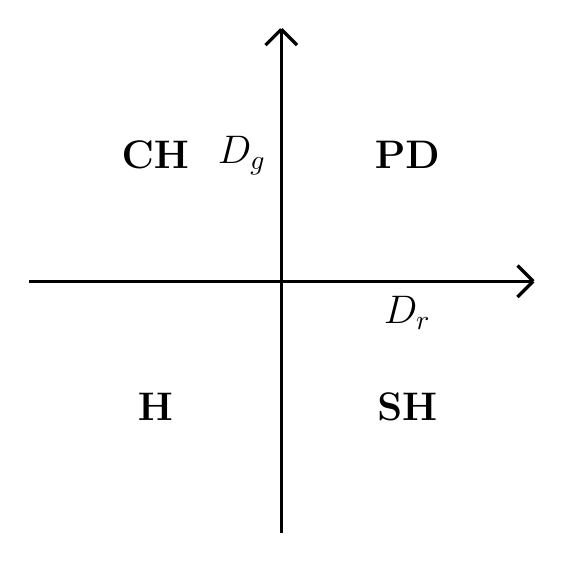
\begin{tikzpicture}

%axis
\draw[very thick] (-3.2,0) -- (3.2,0);
\draw[very thick] (0,-3.2) -- (0,3.2); 

%quiver heads
\draw[very thick] (-0.2,3) -- (0,3.2);
\draw[very thick] (0.2,3) -- (0,3.2);

\draw[very thick] (3,-0.2) -- (3.2,0);
\draw[very thick] (3,0.2) -- (3.2,0);

\draw (-0.5,1.6) node {\Large{$D_g$}};
\draw (1.6,-0.4) node {\Large{$D_r$}};

\draw (-1.6,1.6) node {\Large{\textbf{CH}}};
\draw (1.6,1.6) node {\Large{\textbf{PD}}};
\draw (1.6,-1.6) node {\Large{\textbf{SH}}};
\draw (-1.6,-1.6) node {\Large{\textbf{H}}};

\end{tikzpicture}
    \caption{Diagram representing the four types of pairwise social games according to dilemma strength. CH stands for the Chicken game, PD for the Prisoner's Dilemma, SH stands for the Stag-hunt game and H stands for Harmony game. }
    \label{fig:SocialGames}
\end{figure}


The risk-adverting dilemma strength, together with the gamble-intending dilemma strength $D_g = T - R$ composes the map of types of games pairwise social games represented in Fig.~\ref{fig:SocialGames}. These games are the harmony game, where $D_r,D_g < 0$, no dilemma is found and the logic option is to cooperate; the stag hunt game with, $D_r > 0, D_g < 0$ where the logic option is to do the same as your opponent; the chicken game with $D_r < 0, D_g > 0$, where the logic option is to do the opposite than your opponent; and finally the prisoner's dilemma with $D_r,D_g > 0$ where the logic option is to defect. However if both cooperated they would have better than both defecting but the temptation $T$ is higher than the reward $R$, thus promoting the tragedy of the commons and receiving their punishment $P$~\cite{TragedyCommons}.

Each player is put in a square grid with periodic boundaries, and plays eight games with their Moore neighbors, Fig.~\ref{fig:Moore2Neigh}. Then they sum the payoff gained in all those games and compare the result with their neighbors and copy the strategy of the one with greater total payoff in that round. This is done for all players simultaneously and repeated through time. 


\begin{figure}
\centering
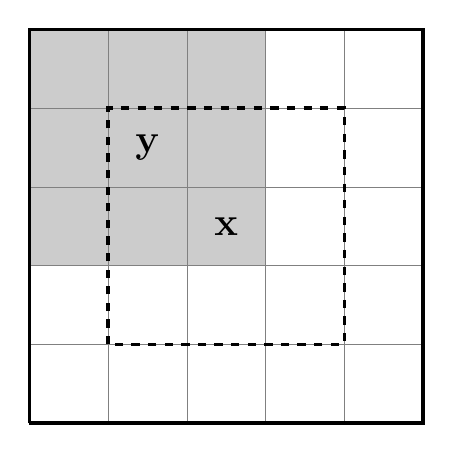
\begin{tikzpicture}


\fill[gray!40!white] (0,2) rectangle (3,5);


\draw[step=1cm,gray,very thin] (0,0) grid (5,5);

\draw[very thick] (0,0) -- (0,5) -- (5,5) -- (5,0) -- (0,0);
\draw[dashed, very thick] (1,1) -- (1,4) -- (4,4) -- (4,1) -- (1,1);

\draw (2.5,2.5) node {\Large{\textbf{x}}};
\draw (1.5,3.5) node {\Large{\textbf{y}}};


\end{tikzpicture}
\caption{Agent $x$'s strategy is affected by the payoff of all agents in his Moore neighborhood (inside the dashed line); for example agent $y$, whose payoff depends of his own Moore neighborhood (shaded region). Therefore, the strategy of the agent $x$ depends on all $25$ agents in his second Moore neighborhood (inside the bold line).}
\label{fig:Moore2Neigh}
\end{figure}





We plot cooperators in blue and defectors in red in Fig.~\ref{fig:PD_Sequencia}. These plots show spatio-temporal chaotic patterns that evolve quickly. In~\cite{SpatialChaos} the authors claimed them to be fractal-like structures. However, as we can see on Fig.~\ref{fig:GranPlot}, when we augment the population size $N$, the patterns do not scale, and instead the clusters all size similarly.




\begin{figure}
    \centering
    \includegraphics[width=0.8\linewidth]{Images/P3/PD_Secuencia.png}
    \caption{Snapshots of the public goods game at $4$ different times of cooperators in blue, defectors in red, and agents that have changed from the previous configuration in yellow. The snapshots are taken at instants $t1 = 1000$, $t2 = 1002$, t3 = $1004$ and $t4 = 1006$ after one defector is introduced at the center in a sea of cooperators in a grid of $101\times101$ agents with periodic boundaries.}
    \label{fig:PD_Sequencia}
\end{figure}


\begin{figure}
    \centering
    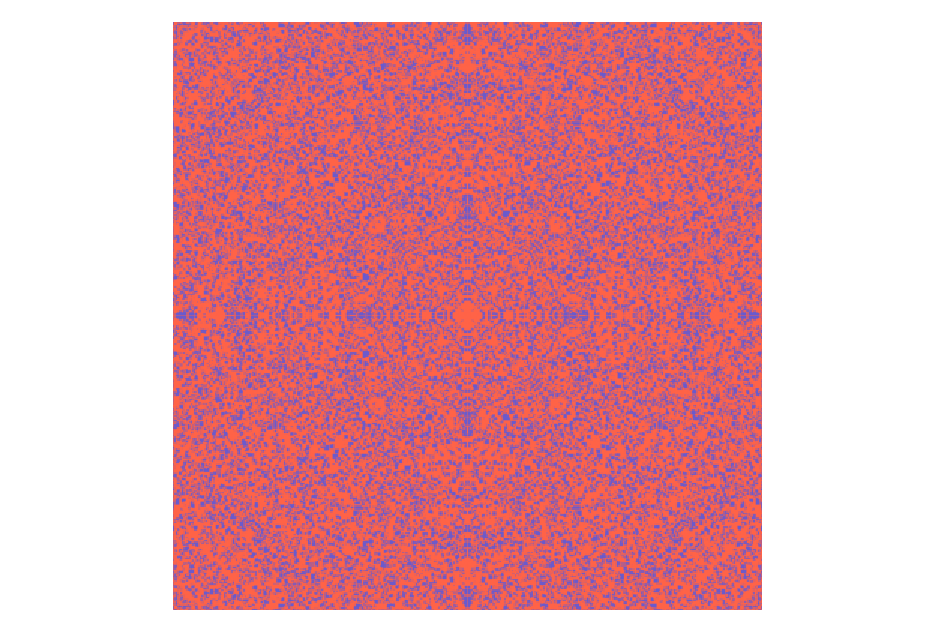
\includegraphics[width=1\linewidth]{Images/P3/PD_GranPlot.eps}
    \caption{Cooperators and defectors in blue and red, respectively.}
    \label{fig:GranPlot}
\end{figure}















The authors of~\cite{SpatialChaos} made an observation that the patterns seemed chaotic for these values of the temptation reward, $1.8 < T < 2$. We want a tool that quantifies the complexity of the pattern evolution that presents spatio-temporal chaos. We think that the algorithm we have developed, described in the following subsection, serves as an indicator for complex behavior and provides a value that quantifies how quickly the patterns evolve, which may be related to the Lyapunov time.



\subsection{Hamming distance measure}


The Hamming distance measures the difference between two objects as the number of different elements they contain. Think of two matrices or vectors of the same size, the Hamming distance between is the number of elements that differ from each position. Now we can represent the configuration of cooperators and defectors at each time as a matrix of $0$'s and $1$'s. Then we can calculate the Hamming Distance of two configurations by subtracting them and taking absolute values since they are binary matrices.

When we do so we observe that the distance quickly goes to zero for simulations in all parameter regimes except for values of the temptation reward in $1.8 < T < 2$, where it growths until it saturates at a given value that augments with population size as we can see in Fig.~\ref{fig:HammingTimePopulation_PD}. We can analytically calculate this value, since it is the statistical Hamming distance, that two random configurations of $0$'s and $1$'s with certain probabilities would have. This value is proportional to the population size, and is calculated as:
\begin{equation}
H_{stat}(t)=N_C(t)p_D(t)+N_D(t)p_C(t),
\end{equation} 
where $N_C$ and $N_D$ indicate the number of cooperators and defectors; and $p_C$ and $p_D$, the proportion of them. Since the proportion of cooperators and defectors is the number of them divided by the total population, we find that the 
proportionality constant for the saturation values of the Hamming distance is
\begin{equation}
h_{stat}(t)=p_C(t)p_D(t)+p_D(t)p_C(t),
\end{equation} 
which, in the case of binary strategies, it can be simplified as:
\begin{equation}
h_{stat}(t)=2p_C(t)(1-p_C(t)).
\end{equation} 

This value could be time dependent, but since the system is stable, the proportions of cooperators and defectors follow the Nash equilibrium and depend only on the values of $T$.



\begin{figure}
	\centering
	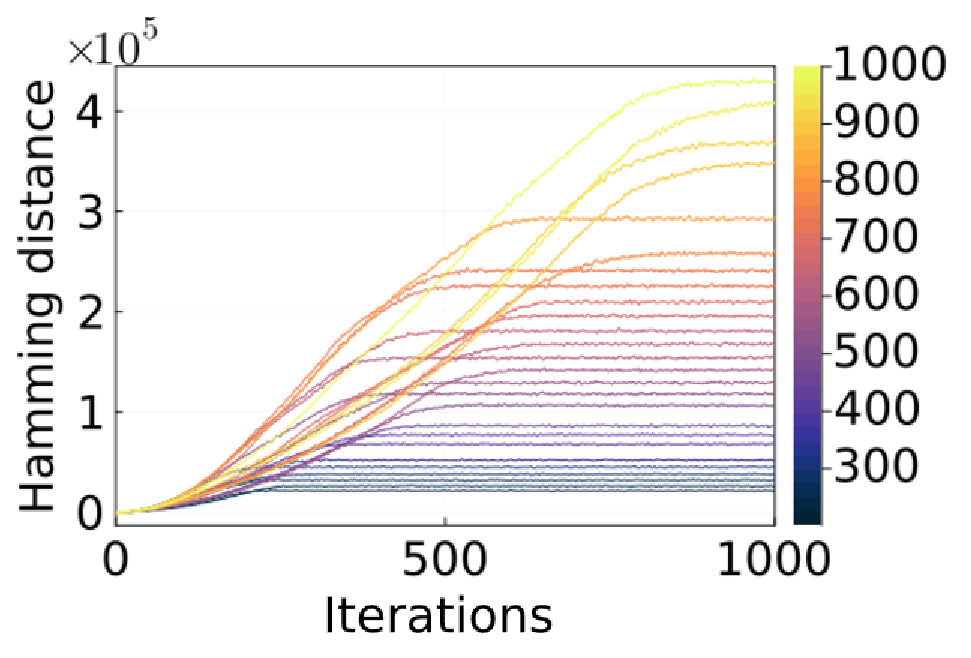
\includegraphics[width=0.8\linewidth]{Images/P3/HammingTimePopulation_PD.eps}
	\caption{Hamming distance of the the two solutions of the prisoner's dilemma versus time. Different colors represent different values of the grid size $L$. The larger the grid size, the longer it takes for the Hamming distance to reach the saturation value $H_{stat}$.}
	\label{fig:HammingTimePopulation_PD}
\end{figure}






Then, if we normalize the Hamming distance from Fig.~\ref{fig:HammingTimePopulation_PD}, dividing it by $H_{stat} = h_{stat}*N$, we get the normalized Hamming distance in Fig.~\ref{fig:NormalHammingTimePopulation_PD}. This figure shows sigmoids with different growth rate. Larger population sizes take longer to reach the saturation value.



\begin{figure}
	\centering
	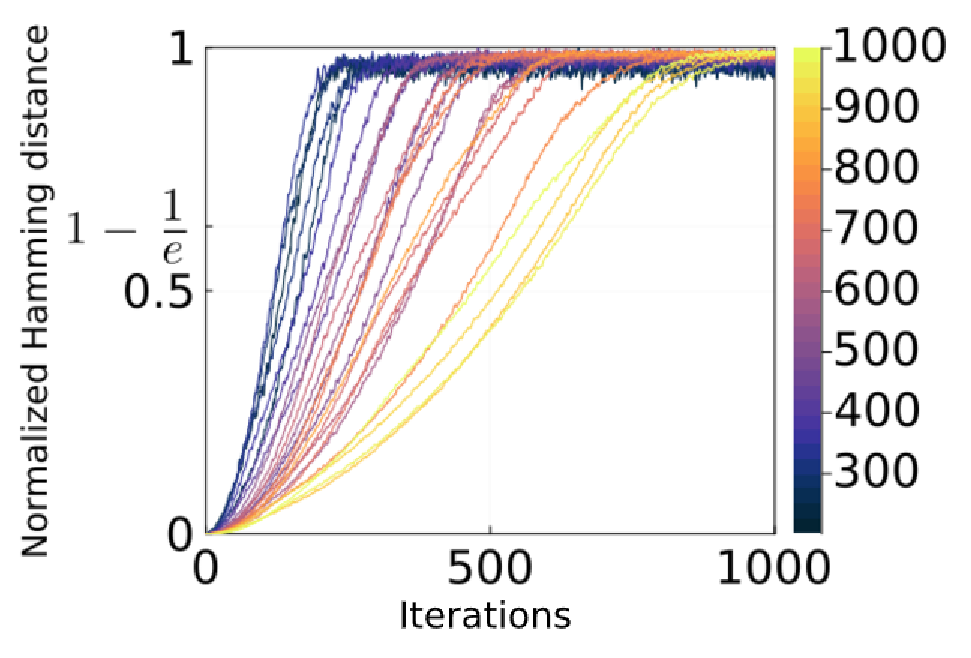
\includegraphics[width=0.8\linewidth]{Images/P3/NormalHammingTimePopulation_PD.eps}
	\caption{ Normalized Hamming distance of the two solutions of the prisoner's dilemma versus time. Multiple curves are shown with different colors, representing the different grid size $L$ values. The curves grow in a sigmoid-like curve towards one. They are normalized to the statistical Hamming distance which depends on L. The larger $L$ is, the longer it takes for the normalized Hamming distance to reach $1$.}
	\label{fig:NormalHammingTimePopulation_PD}
\end{figure}


\begin{figure}
	\centering
	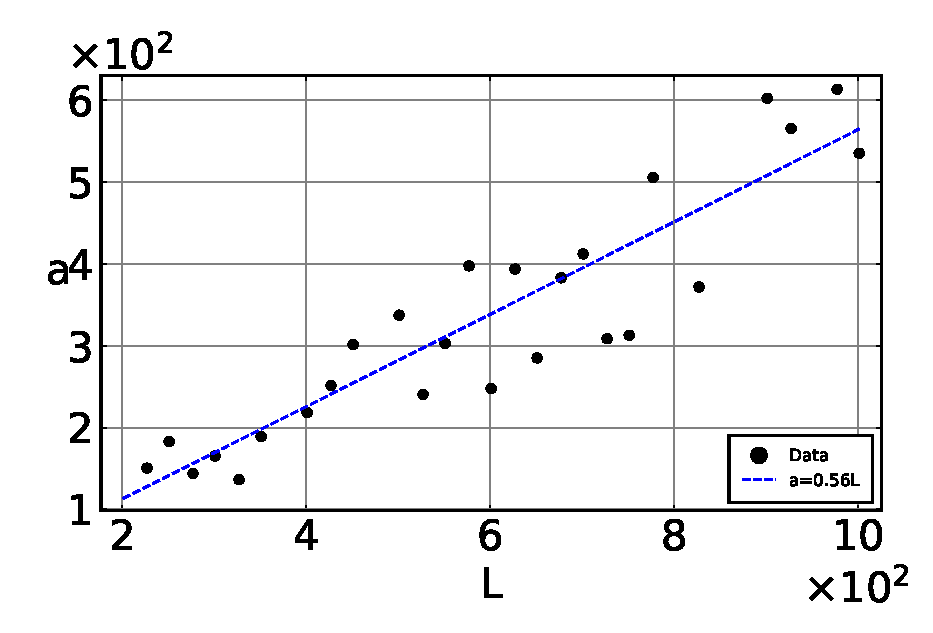
\includegraphics[width=0.8\linewidth]{Images/P3/aVSL_PD.eps}
	\caption{Parameter $a$ from the Weibull ``stretched exponential" function $F(t;k,a)=1-e^{-(t/a)^k}$ fitted to the normalized Hamming distance of the solutions for the prisoner's dilemma versus grid size $L$. It shows a linear regression (dashed blue line) where $a$ grows proportionally to $L$.}
	\label{fig:aVSL_PD}
\end{figure}





We have fitted this curves to the Weibull "stretched exponential" function~\cite{Weibull}
\begin{equation}
    F(t;k,a)=1-e^{-(t/a)^k},
    \label{WeibullDistr}
\end{equation}
where $a$ is the timescale of growth and $k$ tells how abrupt the growth is. We chose this function because it is the most simple sigmoid function that values zero at the origin and converge to one, having only two relevant parameters.

The value of $a$ can be seen as something similar to the Lyapunov time, and as seen on Fig.~\ref{fig:aVSL_PD}, it is proportional to the grid size $L$, with a slope of $0.56 \pm 0.05$ and a neglible intercept. Note that the population size is $N = L^2$. The maximum slope is $0.5$, since at maximum velocity any change in the agent's strategy propagates to two agents away as seen on Fig.~\ref{fig:Moore2Neigh}. The measured value of the slope is near the maximum which indicates a great propagation of the mismatches, and that may be related to complex behavior. As for the values of $k$, every curve is around $k = 2.5\pm0.4$.




\begin{figure}
\centering
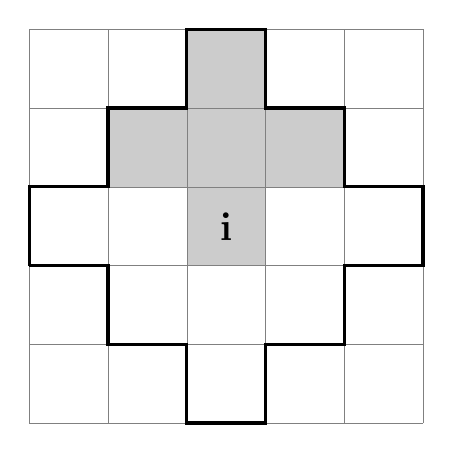
\begin{tikzpicture}

\fill[gray!40!white] (2,2) rectangle (3,5);
\fill[gray!40!white] (1,3) rectangle (4,4);

\draw[step=1cm,gray,very thin] (0,0) grid (5,5);

\draw[very thick] (0,2) -- (0,3) -- (1,3) -- (1,4) -- (2,4) -- (2,5) -- (3,5) -- (3,4) -- (4,4) -- (4,3) -- (5,3) -- (5,2) -- (4,2) -- (4,1) -- (3,1) -- (3,0) -- (2,0) -- (2,1) -- (1,1) -- (1,2) -- (0,2);

\draw (2.5,2.5) node {\Large{\textbf{i}}};


\end{tikzpicture}
\caption{Von Neumann neighborhood at a distance $2$ of agent $i$. The individual $i$ plays $5$ games with agents in cross-like patterns like the one shaded.}
\label{fig:VonNeumman2Neigh}
\end{figure}



\section{Public Goods Game}

Now that we have checked that our algorithm can asses the complexity in the PD, we want to measure weather the game we studied in the previous chapter was chaotic. The public goods game, PGG. 

\subsection{Model}

This time, to make the model simpler we only allow the cooperate and defect strategy, and leave out the punish strategy. The rest of the model we leave the same. That is, agents play $5$ games along $4$ other agents among their second Von Neumann neighbors, Fig.~\ref{fig:VonNeumman2Neigh} and their payoff depends whether they are cooperators, $\Pi_C$, or defectors, $\Pi_D$ and the number of cooperators $N_C^g$ that there are in their group.

\begin{equation}
    \begin{split}
    	&\Pi_C^g=\frac{r}{G}\cdot N_C^g-1 \\
    	&\Pi_D^g=\frac{r}{G}\cdot N_C^g
    \end{split}    
\end{equation}

Here $r$ is a parameter that rewards cooperation and $G = 5$ is the size of the group.

Then, the accumulated payoff $\Pi=\sum_g^G \Pi^g$ determines the fitness of each agent in an evolutionary model where a random agent chooses whether to adopt or not the strategy of a random neighbor. This time we wanted to reduce the stochasticity. Therefore, this time, if the accumulated payoff of the agent's neighbor is greater, it adopts its strategy. Whereas if it is lesser, it does nothing. Nonetheless we still maintained the random election of the agent that will change its strategy to maintain the same game as previous chapter, where the parameter of noise $K$ is in the limit of $K \to 0$.


\begin{figure}
	\centering
	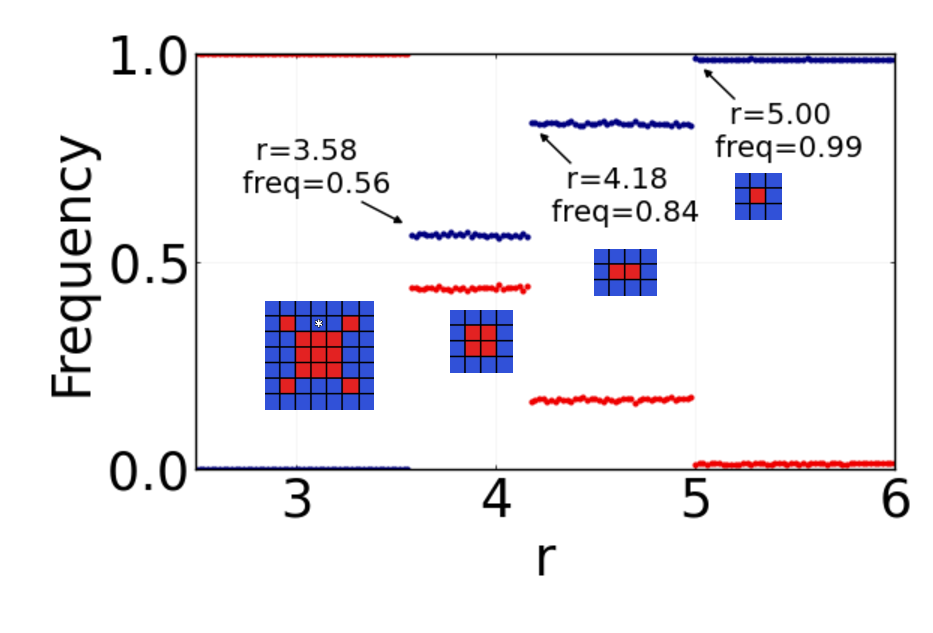
\includegraphics[width=1\linewidth]{Images/P3/PGG_Proportion.eps}
	\caption{Proportion of cooperators (in blue) and defectors (in red) after running a simulation of the public goods game starting with a random strategy in each of the $N=90000$ agents with a relaxation time of $2000$ generations. We can see that the proportion changes only at some values of $r$. This values have been calculated analytically. Each shifts corresponds to a change on whether the surrounding cooperators have greater or lesser payoff than the surrounded defectors in the configurations we show. For the first configuration this holds strictly for the white-marked cooperator and the defector below it at the first shift at $r=25/7\approx3.57$.}
	\label{fig:PGG_Proportion}
\end{figure}


Under these rules, we observe that after a transitory period, the average population stabilizes with  cooperator and defector proportions given by Fig.~\ref{fig:PGG_Proportion}. It shows that the proportion only changes at some values of $r$ and then stays constant. We are able to predict the values of $r$ where these shifts appear analytically. We just have to compare the payoff of the defectors and the cooperators that surround them in configurations that are clusters of defectors of different sizes that are shown in the figure.

As an example here we have the payoff of the white marked cooperator in the first configuration and the defector below it.

\begin{equation}
    \begin{split}
    	&\Pi_C=\frac{1}{5}(5r+4r+2\times3r+r)-5=\frac{16}{5}r-5 \\
    	&\Pi_D=\frac{1}{5}(4r+2\times2r+r+0)=\frac{9}{5}r
    \end{split}
\end{equation}

When we equal these two payoffs we get that the value of $r$ where we expect a shift is $r=25/7\approx3.57$, which is indeed where we find the shift. The next shifts can be calculated similarly with the rest of the configurations and give values of $25/6=4.1\hat6$, $25/5=5$ and $25/3=8.\hat3$.


In the PGG cooperation is a Nash equilibrium for $r\geq5$. At the Nash equilibrium  the payoff cannot be increased when changing strategy given that the rest of agents don't change theirs. But we observe that for $5<r<8.\hat3$ cooperation is not the only strategy present. This is because the payoff of each agent is affected by the strategies of its neighbors. Therefore, a defector surrounded by cooperators has greater payoff than them, even though it would have greater payoff if it were a cooperator. This means that being at a Nash equilibrium does not eliminate all defectors. We observe a last shift at $r=8.\hat3$, beyond this last shift defection is not viable.  We don't show this shift in Fig.~\ref{fig:PGG_Proportion} because it can hardly be appreciated at the current scale (from a cooperator proportion of $0.99$ to $1$). What's more, since the election of the agent that changes its strategy is at random, the computational times for all defectors to adopt the cooperation strategy are large.





\subsection{Hamming distance measure}




\begin{figure}
    \centering
    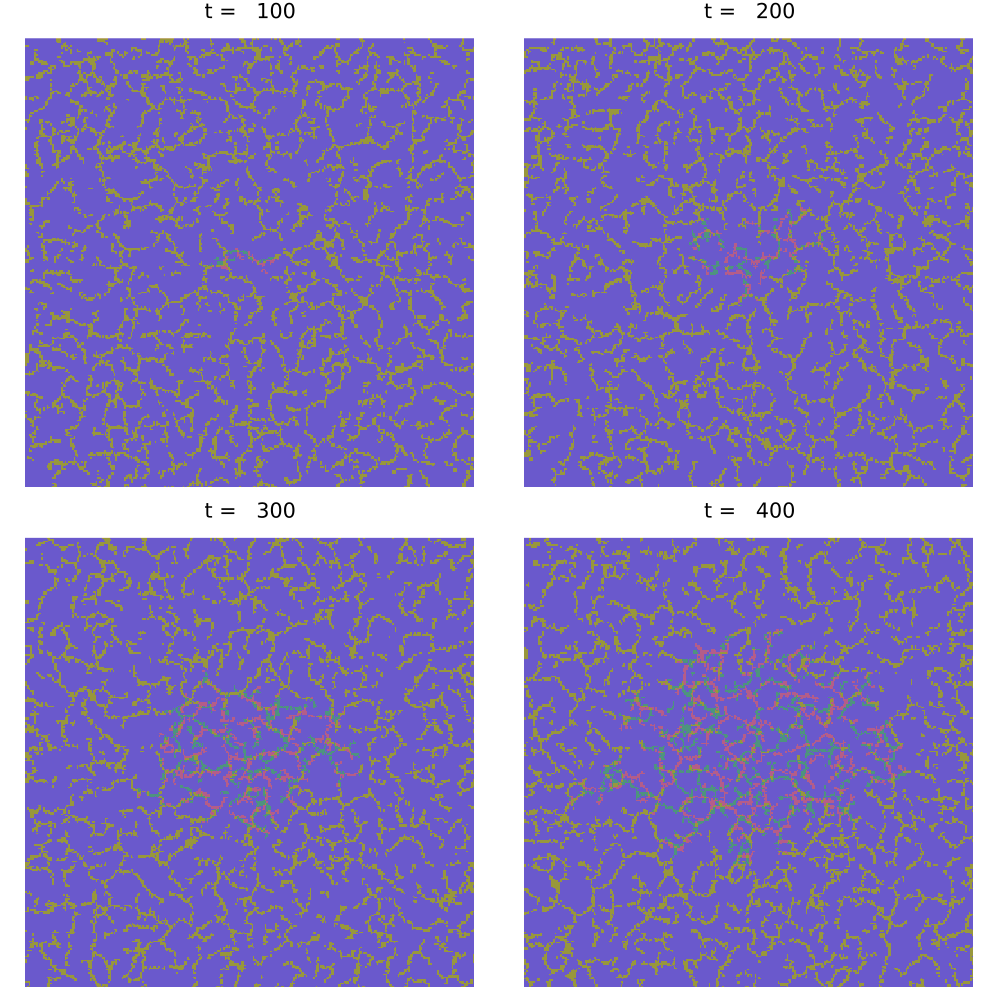
\includegraphics[width=0.8\linewidth]{Images/P3/PGG_SecuenciaHamming.png}
    \caption{Snapshots at $4$ different times of both configurations (original, and copy with altered agent at $t = 0$ at the center) of the public goods game. Cooperators are plotted in blue, defectors in red for one configuration and in green for the other. Both configurations are plotted one on top of the other with a transparent effect. Thanks to this we can see that the mismatches propagate at average constant velocity and expand radially.}
    \label{fig:PGG_SequenciaHamming}
\end{figure}





\begin{figure}
	\centering
	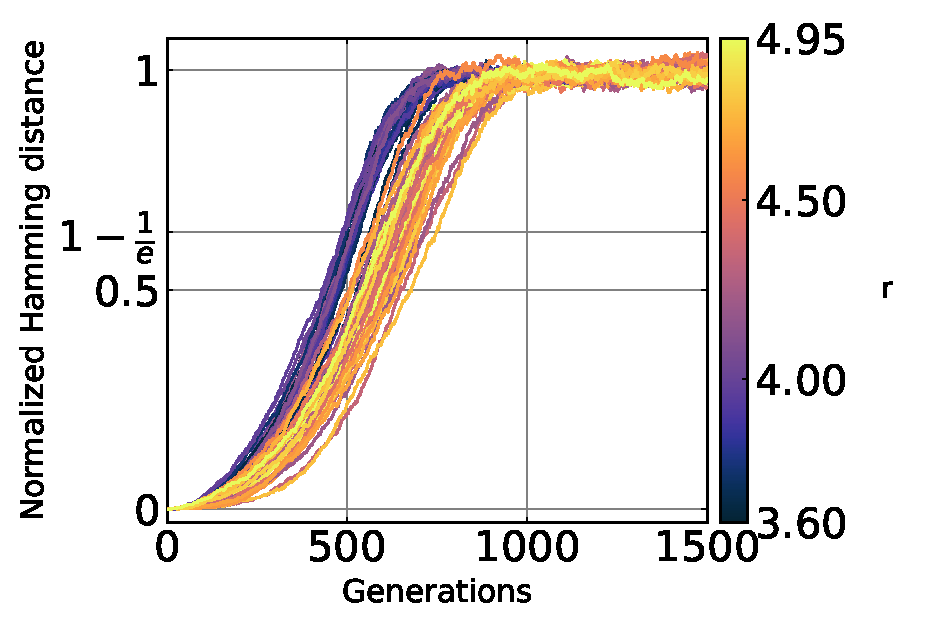
\includegraphics[width=1\linewidth]{Images/P3/NormalHammingTimePopulation_r.eps}
	\caption{Normalized Hamming distance between the solutions for the public goods game versus time. Multiple curves are shown with different colors, representing the different $r$ values. The curves grow in a sigmoid-like curve towards one. They are normalized to the statistical Hamming distance, which depends on $r$, so curves ranging from  $25/7\leq r<25/6$ are normalized to a different value than those at $25/6\leq r<5$. There is a distinction between the two regimes, the curves of the first one (blue ones) reach its midpoint earlier than the ones in the second regime (orange ones).}
	\label{fig:NormalHammingTimePopulation_r}
\end{figure}



\begin{figure}
	\centering
	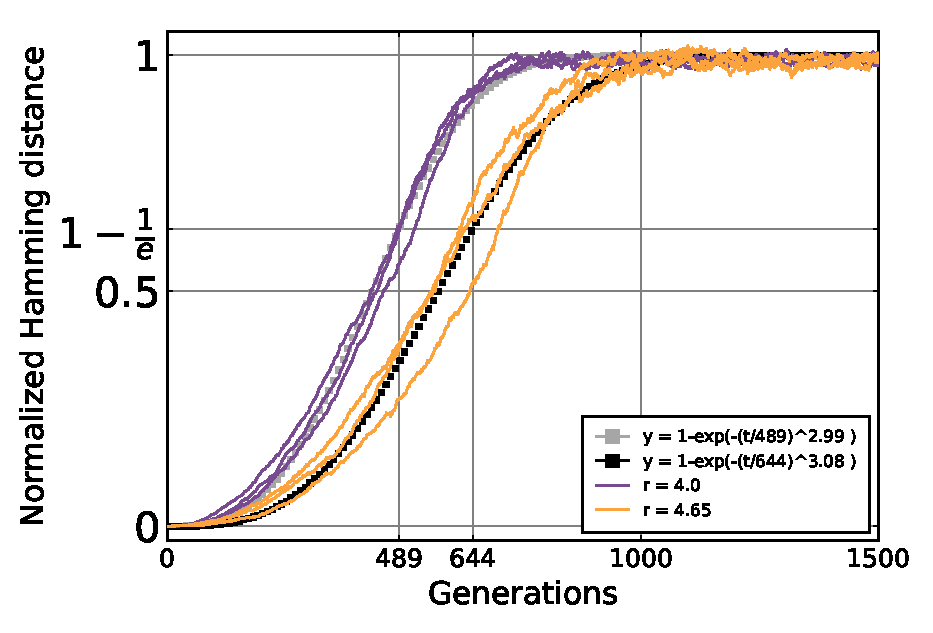
\includegraphics[width=1\linewidth]{Images/P3/NormalHammingTimePopulation_2r.eps}
	\caption{Normalized Hamming distance between the solutions for the public goods game versus time. Different colors represent two different $r$ values. They are normalized to the statistical Hamming distance, which depends on $r$, so the two curves are normalized to a different value. The Weibull ``stretched exponential" function $F(t;k,a)=1-e^{-(t/a)^k}$ is fitted to the curves and we observe different values of $a$, which can be seen as similar to the Lyapùnov time. The $r=4$ curves (blue and left ones), representing the regime $25/7\leq r<25/6$ has a lower value of $a$ than the curves with $r=4.65$ (orange and right ones). This indicates that, for $25/7\leq r<25/6$, the system is more sensitive to initial conditions.}
	\label{fig:NormalHammingTimePopulation_2r}
\end{figure}




To asses the complexity of our PGG we measured the Hamming distance of two initially close configurations differing of only one agent. Because the election of the agent that adopt a new strategy in the evolutionary model is chosen at random, we have to make sure every random interaction is chosen the same through both simulations.


We can see how mismatches propagate in Fig.~\ref{fig:PGG_SequenciaHamming}. For each snapshot both configuration, the original and the copy with a different agent at the center, are plotted on the same space in two layers with one layer being slightly transparent. The defectors in one configuration are ploted red and in the other, green. This allows us to watch how the mismatches propagate. They do so radially and at constant velocity on average, but following the branches of defectors when watched closely.



The result was, as seen in Fig.~\ref{fig:NormalHammingTimePopulation_r} that the Normalized Hamming distance grew as a sigmoid like in the previous section for values of the parameter $r$ between $25/7\approx3.57$ and $8.\hat3$. These are all the values where there are present cooperators and defectors . We cannot say that this is an indicator of chaos this time, because probably, what the algorithm is assessing is the randomness in the election of agent to change its strategy. Nonetheless, when we fit the curves to the Weibull ``stretched exponential" function in Fig.~\ref{fig:NormalHammingTimePopulation_2r}, we get lower values of $a$ for curves in the first regime, $25/7\leq r<25/6$. This means that the system is more susceptible to changes in the initial conditions. For values of $5>r>8.\hat3.$ we get a very large value of $a = 3685$.


\section{Discussion and conclusions}

We have developed an algorithm to measure the divergence of two binary configurations of cooperators and defectors in the prisoner's dilemma and the public goods game using the Hamming distance. We observed that if the game has no random elements, the divergence can be linked to complex behavior.
The Hamming distance grew as a sigmoid function in time for a system that was clear, had a complex behavior and was zero when not.
 
We also calculated a measure that could correlate to a Lyapunov time. The measure, which indicated approximately the midpoint of the sigmoids, was proportional to the grid size and the constant of proportionality was near its maximum for the prisoner's dilemma with no random elements.

For the public goods game with some random elements, all games studied presented a divergence of the Hamming distance. Nonetheless, the divergence was slower, it took longer to reach the midpoint, for some games, which had a sparse population of defectors and a great number of cooperators.

Even though our studied was focused on two particular cases, we are sure the algorithm is adequate to measure divergence and stability in many systems and geometries due to the simplicity of its implementation. In fact, in the next chapter we explain how we used the same tool to make a classification of elementary cellular automata based on complexity.

 




\begin{thebibliography}{04}



\bibitem{SpatialChaos}
M. A. Nowak and R. M. May,
Evolutionary games and spatial chaos. 
Nature \textbf{359}, 826--829 (1992).
\url{https://doi.org/10.1038/359826a0}

\bibitem{HammingOrigins}
\raggedright
R.Hamming,
Error detecting and error correcting codes.
Bell Syst. Tech. J. \textbf{29}, 147--160 
(1950).
\url{https://doi.org/10.1002/j.1538-7305.1950.tb00463.x}


\bibitem{HammingSocial1}
\raggedright
R. D'hulst and G. J. Rodgers,
The hamming distance in the minority game.
Physica A \textbf{270}, 514--525 (1999). 
\url{https://doi.org/10.1016/S0378-4371(99)00211-3}

\bibitem{HammingSocial2}
\raggedright
J.-W. Kim,
A tag-based evolutionary prisoner's dilemma game on networks with different topologies.
JASSS, \textbf{13}, 2 (2010).
\url{https://doi.org/10.18564/jasss.1584}

\bibitem{HammingChaos1}
\raggedright
D. Bazeia, M. B. P. N. Pereira, A. V. Brito, B. F. Oliveira, and J. G. G. S. Ramos,
A novel procedure for the identification of chaos in complex biological systems.
Sci. Rep. \textbf{7}, 44900 (2017).
\url{https://doi.org/10.1038/srep44900}

\bibitem{HammingChaos2}
\raggedright
D. Bazeia, J. Menezes, B. F. De Oliveira, and J. G. G. S. Ramos,
Hamming distance and mobility behavior in generalized rock-paper-scissors models.
EPL \textbf{119}, 58003 (2017).
\url{https://doi.org/10.1209/0295-5075/119/58003}

\bibitem{TragedyCommons}
\raggedright
G. Hardin,
The tragedy of the commons: the population problem has no technical solution; it requires a fundamental extension in morality.
Science \textbf{162}, 1243--1248 (1968).
\url{https://doi.org/10.1126/science.162.3859.1243}


\bibitem{Weibull}
\raggedright
W. Weibull, A statistical distribution function of wide applicability.
J. Appl. Mech. \textbf{18}, 293--297 (1951).
\url{https://hal.science/hal-03112318v1}
\end{thebibliography}
